\documentclass[10pt, a4paper,titlepage]{article}

\usepackage{graphicx}
\usepackage{tabularx}
\usepackage{listings}
\usepackage[normalem]{ulem}
\usepackage{caption}
\usepackage[bottom]{footmisc}
\usepackage{textcomp}
\usepackage{amsmath}

\begin{document}
\begin{titlepage}
\title{Project Plan Document\\Version 1.0}
\author{Emanuele Ricciardelli (mat. 875221) \and Giorgio Tavecchia (mat. 874716) \and Francesco Vetr\'o (mat. 877593)}
\begin{figure}
\begin{center}

\includegraphics{/home/francesco/git/Project_SE2_RTV/Project_Plan/PP_images/logopolimi.png}
\caption{Politecnico di Milano}
\label{fig:logo}
\end{center}
\end{figure}
\maketitle
\end{titlepage}
\tableofcontents
\pagebreak
\section{Introduction}
\subsection{Purpose and scope}
The purpose of this document, the Project Plan, is to analyze the complexity of the PowerEnJoy system in order to make a more accurate prediction of the costs and efforts necessary for the development of all the components of the system.
These data will then be useful to define budget, schedule and subdivision of resources and tasks within the team.
This document will be structured in 3 macro parts:
\begin{itemize}
\item The first section will deal with the analysis necessary to define an estimate of the size of the project, in function of lines of code, as well as the cost / effort. This analysis will be conducted in terms of Function Points and COCOMO II approach.
\item The second section will present a schedule for the project so as to ensure a proper distribution of tasks and times in order to achieve all of the system requirements, implementation and testing aspects.
\item In the third section we will discuss about risk management, through an analysis of possible problems that may arise during the development and the applicable remedies.
\end{itemize}•
\subsection{Definitions and abbreviations}
\begin{itemize}
\item RASD: Requirement Analysis and Specification Document.
\item DD: Design Document
\item ITPD: Integration Test Plan Document
\item PM: person-months
\item KSLOC: kilo-source lines of code
\item ILF: Internal Logic Files
\item ELF: External Interface Files
\item EQ: External Inquiries
\item EI: External Inputs
\item EO: External Output
\end{itemize}
\subsection{Reference documents}
\begin{itemize}
\item Specification document: Assignments AA 2016-2017.pdf
\item RASD Version 1.1    
\item DD Version 1.1
\item ITPD Version 1.0
\item Project planning example document.pdf
\item Function Point Languages Table: \emph{http://www.qsm.com/resources/function-point-languages-table}
\item CII\_modelman2000.0.pdf
\end{itemize}
\section{Project size, cose and effort estimation}
This section will focus on providing an estimate of the size of the system that will be, as well as costs and development efforts.
Regarding the estimate of the size of the future system, we will make use of Function Point which will allow us to make an estimate based on the features that the system will have to offer.
Concerning the estimated costs and effort related to the development, we will make use of COCOMO II and we will integrate the results previously obtained.
\subsection{Size estimation: function points}
In this chapter we will face an approach through Function Point in order to estimate the size of the system to be developed, using as a unit of measurement the KSLOC.
In particular, we are going to make a calculation of all the Function Points of the system, by the following equation:
\begin{center}
UFP = $\sum$ (\# elements of a given type $\times$ weight)
\end{center}
The possible types of elements affecting the expression concern:
\begin{itemize}
\item Data structure;
\item Inputs and outputs;
\item Inquiries;
\item External Interface.
\end{itemize}
We provide a definition for each of them in the relevant section.
While, with respect to the definition of the weights, we are going to use the following table, which allows us to define, for each element, the weight as a function of the inherent complexity of its implementation.
\begin{table}[h]
\caption{Complexity weight}
\begin{tabularx}{\textwidth}{|>{\hsize=.4\hsize}X|>{\hsize=.2\hsize}X|>{\hsize=.2\hsize}X|>{\hsize=.2\hsize}X|}
\hline
Function type & Low & Average & High\\ 
\hline
Internal Logic Files & 7 & 10 & 15\\
\hline
External Interface Files & 5 & 7 & 10\\
\hline
External Inputs & 3 & 4 & 6\\
\hline
External Inquiries & 3 & 4 & 6\\
\hline
External Outputs & 4 & 5 & 7\\ 
\hline
\end{tabularx}
\end{table}
\subsubsection{Internal Logic Files (ILFs)}
With Internal Logic Files we define internal data generated by
the system, and used and maintained by it. This set contains homogenous data handled by the system, composed by all the data structure saved in the DBMS.
In the list below we list the tables which compose our database. They fill the Internal Logic Files set.
\begin{itemize}
\item User(\underline{Password}, email, name, surname,drivingLicenseNumber)
\item Reservation(\underline{ID,userPassword,licensePlateCard}, date,startingTime,endingTime)
\item Car(\underline{licensePlate}, model)
\item MaintenanceRecord(\underline{ID},description,date, licensePlate)
\item Sensor(\underline{ID}, licensePlate)
\item ExtraInRes(\underline{ID, IDextra, IDreservation})
\item Extras(\underline{ID}, type, value)
\item Payment(\underline{prog\_number, IDReservation}, pending, date)
\item Ride(\underline{ID}, IDReservation, startingTime, endingTime, bill, lastBatteryLevel,date, startingSafeArea, endingArea)
\item Ticket(\underline{IDTicket, IDRide}, date)
\item Area(\underline{ID}, position)
\item SafeArea(\underline{IDArea})
\item UnsafeArea(\underline{IDArea})
\item PowerGrid(\underline{ID}, capacity, IDSafeArea)
\item BonusMalus(\underline{ID}, amount, description)
\item AssignedBonusMalus(\underline{IDRide, IDBonusMalus})
\end{itemize}
With respect to the previous table of complexity weight, we decide to assign a \emph{LOW} level to those tablet that are composed by a small number of attributes, while we define as \emph{AVERAGE} level of complexity tables such as Reservation that is derived from the interaction of multiple tables. For the same reason, but with an higher level of complexity, we assign to the Ride table the \emph{HIGH} level.
\begin{table}[h]
\caption{ILFs}
\begin{tabularx}{\textwidth}{|>{\hsize=.5\hsize}X|>{\hsize=.25\hsize}X|>{\hsize=.25\hsize}X|}
\hline
ILF & Complexity Level & FPs\\ 
\hline
User & Low & 7\\
\hline
Reservation & Avg & 10\\
\hline
Car & Low & 7\\
\hline
Maintenance Record & Low & 7\\
\hline
Sensor & Low & 7\\
\hline
ExtraInRes & Low & 7\\
\hline
Extras & Low & 7\\
\hline
Payment & Low & 7\\
\hline
Ride & High & 15\\
\hline
Ticket & Low & 7\\
\hline
Area & Low & 7\\
\hline
Safe Area & Low & 7\\
\hline
Unsafe Area & Low & 7\\
\hline
Power Grid & Low & 7\\
\hline
BonusMalus & Low & 7\\
\hline
AssignedBonusMalus & Low & 7\\
\hline
& TOT & 123\\
\hline
\end{tabularx}
\end{table}
\pagebreak
\subsubsection{External Interface Files (EIFs)}
With External Interface Files we identify a set of data used by the PowerEnJoy system that are not stored in it but provided and handled by external companies.
With respect to the PowerEnJoy service, the external data are provided by Google Services and in particular by Google Maps.
The services above, are used by our system making use of the API provided by Google itself. Features requiring their use are as follows:
\begin{itemize}
\item Provide directions, given the current position of a car, to a charging station.
\end{itemize}
This functionality is implemented in the Money-Saving option, in which the user is able to enter their destination and the system returns the location of the nearest charging station to the destination, providing at the same time a uniform distribution of cars in the city; this position will later be used by the API to calculate the optimal route and return there.
Given the complexity of the operations involved (especially those linked to the uniform distribution of cars in the city) we identify this feature as a \emph{AVG} complexity.
\begin{table}[h]
\caption{ELFs}
\begin{tabularx}{\textwidth}{|>{\hsize=.5\hsize}X|>{\hsize=.25\hsize}X|>{\hsize=.25\hsize}X|}
\hline
ELF & Complexity Level & FPs\\ 
\hline
Money saving option & Avg & 7\\
\hline
\end{tabularx}
\end{table}
\pagebreak
\subsubsection{External Inputs (EIs)}
With External Input we identify a set of elementary operation to elaborate data coming from
the external environment.
As defined in previous documents, our system interfaces with a number of clients aimed at different types of users, in particular we will have functionality addressed to users of car sharing service, the maintenance system and the payment system.
In particular for each of them we will provide the following functionalities:
\begin{itemize}
\item Users of the car sharing service:
\subitem - Login/Logout: the login and logout are key features to our system but there are translated into simple queries on the database, which is why the level of complexity is \emph{LOW}.
\subitem - Registration: the registration system is also based on a number of queries on the database, to which, however, are added a series of controls regarding the information entered, the validity of the license provided and the accuracy of data relating to the method of payment chosen. Despite this, it remains a \emph{LOW} complexity.
\subitem - Reserve a car: booking a car is a complex operation that requires a series of queries, followed by several controls both the user (Eg. check if it is suspended) and the selected car (Eg. make sure it is available) and finally a communication with the vehicle to inform the reservation. the multiplicity of the transactions underlying the achievement of this feature allows us to indicate it as a \emph{AVG} complexity.
\subitem - Delete a reservation: linear operation and \emph{LOW} complexity since it corresponds to the simple closure of the reservation and the consequent reflection on the database.
\subitem - Extend a reservation: the operations involved are the same as the \emph{Delete a reservation}, the only addition corresponds to the operations necessary to register the payment due to the extension itself. For this reason, the level of complexity is \emph{LOW}.
\subitem - Start a ride: the operation to \emph{start a ride} requires an exchange of information between the car and the system, in particular the operation can begin when the system validates the unlock code used on the car and the engine is ignited. The underlying operations of this feature affect several components that are going to instantiate different entity in the database. For these reason we define an \emph{AVG} complexity.
\subitem - End a ride: like the previous functionality, are involved different components and entities in the database. the complexity, also in this case, is \emph{HIGH} because the system does not only apply queries on the database but compute all the necessary element to end a ride, like computing the payment and various discounts. This functionality is more complex than “Start a Ride” because in order to fulfill its task, it requires the product of more subprocesses like computing the total amount, performing the payment instantiation, unreserved the car and so on.
\subitem Report a issue: reporting a problem to a car, it may seem a simple task since it requires only the creation of a new “record maintenance”, but underneath  resides the management of the whole reservation or ride that interested the machine. for this reason the average complexity is \emph{AVG}. 
\item Maintenance system:
\subitem - Update a record about a car: the status update concerning a record of a car by the maintenance is a simple task that requires only to update tuples in the database related to the reported car. The complexity is \emph{LOW}.
\item Payment system:
\subitem - Update payment informations: just as in the case of update by maintenance, the only operation involved  is upgrading tuples in the database for a specified payment. The complexity is \emph{LOW}.
\end{itemize}
\begin{table}[h]
\caption{EIs}
\begin{tabularx}{\textwidth}{|>{\hsize=.5\hsize}X|>{\hsize=.25\hsize}X|>{\hsize=.25\hsize}X|}
\hline
EI & Complexity Level & FPs\\ 
\hline
Login/Logout & Low & 3$\times$2=6\\
\hline
Registration & Low & 3\\
\hline
Reserve a Car & Avg & 4\\
\hline
Delete reservation & Low & 3\\
\hline
Extend reservation & Low & 3\\
\hline
Start ride & Avg & 4\\
\hline
End ride & High & 6\\
\hline
Report issue & Avg & 4\\
\hline
Update record car & Low & 3\\
\hline
Update payment information & Low & 3\\
\hline
& TOT & 39\\
\hline
\end{tabularx}
\end{table}
\pagebreak
\subsubsection{External Inquiries (EQs)}
With External Inquiries we define a set of elementary operation that involves input and output operations. With regard to this definition and using the previous subdivision related to different users of the system, we provide the following functionalities:
\begin{itemize}
\item Users of the car sharing service:
\subitem - Retrieve information about his reservation
\subitem - Retrieve unlock code: the previous two steps possess the same level of complexity as they are the result of a simple query to the database, for this reason, is associated to them a \emph{LOW} complexity.
\subitem - Retrieve payment history: since the payment-related information is obtained through analysis of all the costs relating to reservations and ride (e.g. the extension of a reservation or the application of discounts), the complexity of this operation is \emph{AVG}.
\subitem - View available cars: the identification of available cars is the result of an analysis of the non-reserved cars or currently in use /in  maintenance. For this reason, the complexity is \emph{LOW}.
\item Maintenance system:
\subitem - Retrieve a list of reported issue: as well as retrieving information associated with a reservation, cited above, retrieving reports is a simple task, result of an equally simple database query. Complexity \emph{LOW}. 
\end{itemize}
\begin{table}[h]
\caption{EQs}
\begin{tabularx}{\textwidth}{|>{\hsize=.5\hsize}X|>{\hsize=.25\hsize}X|>{\hsize=.25\hsize}X|}
\hline
EQ & Complexity Level & FPs\\ 
\hline
Retrieve reservation info & Low & 3\\
\hline
Retrieve unlock code & Low & 3\\
\hline
Retrieve payment history & Avg & 4\\
\hline
View available cars & Low & 3\\
\hline
Retrieve list of reported issues & Low & 3\\
\hline
& TOT & 16\\
\hline
\end{tabularx}
\end{table}
\pagebreak
\subsubsection{External Outputs (EOs)}
With External Output we define functionalities that our system perform and generate data to the output. 
With respect to this definition, we can define the following functionalities:
\begin{itemize}
\item Notify a user for the correct registration;
\item Notify a user that a reservation has been performed;
\item Notify a user if the car reserved is no longer available;
\item Notify a user for the payment of a ride;
\item Notify the maintenance system if a new issue is reported;
\item Notify the payment system if a new debt is created.
All the notifications listed above are considered simple and for this reason the \emph{LOW} complexity.
\end{itemize}
\begin{table}[h]
\caption{EOs}
\begin{tabularx}{\textwidth}{|>{\hsize=.5\hsize}X|>{\hsize=.25\hsize}X|>{\hsize=.25\hsize}X|}
\hline
EO & Complexity Level & FPs\\ 
\hline
Notify correct registration & Low & 4\\
\hline
Notify performed reservation & Low & 4\\
\hline
Notify car no longer available & Low & 4\\
\hline
Notify payment & Low & 4\\
\hline
Notify new issue & Low & 4\\
\hline
Notify new debt & Low & 4\\
\hline
& TOT & 24\\
\hline
\end{tabularx}
\end{table}
\pagebreak
\subsubsection{Overall estimation}
Given the following summary table:
\begin{table}[h]
\caption{Summary}
\begin{tabularx}{\textwidth}{|>{\hsize=.5\hsize}X|>{\hsize=.5\hsize}X|}
\hline
Function type & Value\\ 
\hline
Internal Logic Files & 123\\
\hline
External Interface Files & 7\\
\hline
External Inputs & 39\\
\hline
External Inquiries & 16\\
\hline
External Outputs & 24\\
\hline
Total & 209\\
\hline
\end{tabularx}
\end{table}
\linebreak
\begin{center}
LOC=AVC$\times$number of function points
\end{center}
Considering Java Enterprise Edition as the development platform, we can assign the value AVC  following the Function Point Language Table linked in the document references.
For the average number of SLOC AVC is equal to 46: 
\begin{center}
SLOC= 209$\times$46= 9614
\end{center}
For the computing an upperbound for the number of SLOC AVC is equal to 67:
\begin{center}
SLOC=209$\times$67=14003
\end{center}
\subsection{Cost and effort Estimation: COCOMO II}
In this section, as previously expressed in the purpose of the document, we will use the COCOMO II approach in order to estimate cost and effort needed to develop the PowerEnJoy system. In particular we will focus on a Post-Architecture approach since we have already detailed informations about the different phases of development, and so we can achieve a more accurate cost estimate.
We now provide an accurate analysis of all the elements needed to perform the following effort equation:
\begin{center}
PM=A$\times$Size$^E\times\prod_{1<=i<=n}EM_i$
\end{center}
In particular, the meaning of the coefficients is the following:
\begin{itemize}
\item A: It’s an approximation of the productivity constant in PM/KSLOC. This coefficient is standardly set to 2.94;
\item Size: is the estimated size of the project in KSLOC, provided in the previous chapter;
\item $EM_i$: effort multiplier, derived for each cost driver;
\item E: is an aggregation of five Scale Factors.
\end{itemize}
\subsubsection{Scale factors}
The first parameter that we will estimate is \emph{E}, obtained by the following equation, a function of scale factors that we will soon identify.
\begin{center}
E=B+0.01$\times\sum_{1<=j<=5}SF_j$
\end{center}
Where B is set to 0.91, as an empirically-proven quantity for COCOMO II.
Regarding $SF_j$, each member of the summation is equivalent to a coefficient of the following table, chosen in function of the range of verylow-extrahigh values, characteristic of each of them.
\begin{figure}[h]
\begin{center}
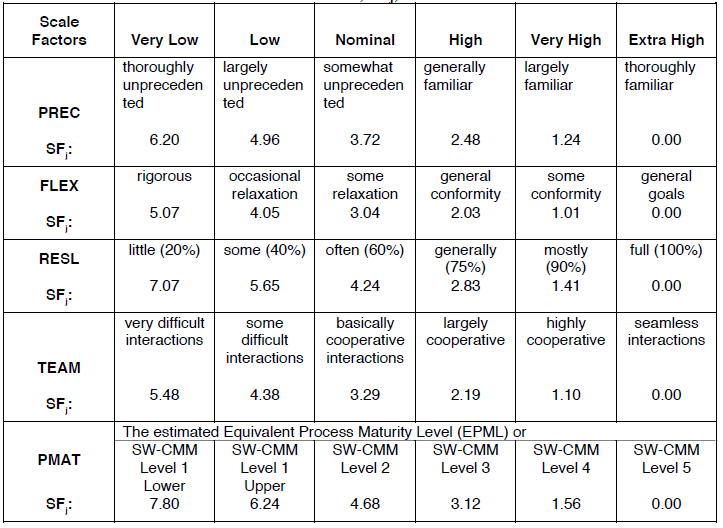
\includegraphics[width=\textwidth, height=0.8\textheight, keepaspectratio]{/home/francesco/git/Project_SE2_RTV/Project_Plan/PP_images/scale_factors.png}
\caption{Scale Factors}
\label{fig:scale}
\end{center}•
\end{figure}
\pagebreak
\linebreak
For each of these factors, we will now provide a definition and the reasoning behind the chosen value:
\begin{itemize}
\item \underline{\textbf{Precedentedness (PREC)}}:  The value of this coefficient decreases much higher is the degree of experience that the team presents in respect of a similar project. In particular, our experience level is \emph{LOW} because we have not previously participated in the development of systems of this size.
\item \underline{\textbf{Development Flexibility (FLEX)}}: The degree of development flexibility reflects the flexibility that the project can presents regarding the requirements and objectives on which it was founded. The PowerEnJoy system has been defined in relation to requirements for the car sharing service that have stiffness from the point of view of the required functionality, with little choice margin, while from the architectural point of view is more flexible since there are no systems legacy to which it is necessary to integrate, but, at the same time, the type of service involves the development of an architecture able to ensure certain levels of operations. For this reason, we assign a \emph{NOMINAL} value.
\item \underline{\textbf{Risk Resolution (RSL)}}: This factor reflects the ability of the development team to recognize and react promptly to the risks and problems that it could be encountered along the development. Also in relation to the same subject discussed in detail in the final chapter of this document, we assign the value \emph{HIGH}.
\item \underline{\textbf{Team Cohesion (TEAM)}}: The Team Cohesion scale factor accounts for the sources of project turbulence and entropy because of difficulties in synchronizing the project’s stakeholders: users, customers, developers etc. These difficulties may arise from differences in stakeholder objectives and cultures, difficulties in reconciling objectives and developer’s lack of experience and familiarity in operating as a team. With respect to this definition we can assign a \emph{VERY HIGH} level, since the development team is collaborative and open to dialogue.
\item \underline{\textbf{Process Maturity (PMAT)}}: This factor is directly linked with the CMMI index, in particular, related to our system, the development project has been properly managed, planned and executed with stakeholders involved and resources rightly distributed. For this rationale, we assign a Level 2, so a \emph{NOMINAL} factor. 
\end{itemize}
\pagebreak
We can now compute the previously presented equation:
\begin{table}[h]
\caption{Scale Factor}
\begin{tabularx}{\textwidth}{|>{\hsize=.5\hsize}X|>{\hsize=.25\hsize}X|>{\hsize=.25\hsize}X|}
\hline
Scale Factor & Factor & Value\\ 
\hline
Precedentedness (PREC) & Low & 4.96\\
\hline
Development Flexibility (FLEX) & Nominal & 3.04\\
\hline
Risk Resolution (RSL) & High & 2.83\\
\hline
Team Cohesion(TEAM) & Very High & 1.10\\
\hline
Process Maturity (PMAT) & Nominal & 4.68\\
\hline
&  & 16.61\\
\hline
\end{tabularx}
\end{table}
\linebreak
Using the previously defined equation:
\begin{center}
E= 0.91+0.01$\times$16.61=1.0761
\end{center}
\subsubsection{Cost drivers}
We now carry out an analysis of the Cost Drivers in order to estimate the value of EM in the equation at paragraph 2.2.
As previously indicated, we will use a post-architecture approach, thus providing an accurate computation of the relative cost drivers.
\begin{itemize}
\item \underline{\textbf{Analyst Capability (ACAP)}}: This driver measures the degree of reliability of the estimates and analyzes which have been carried out for the design of the project. In relation to PowerEnJoy system, we can claim to have performed a detailed analysis not only of the features to be implemented, but also about the environment in which the system have to operate, also investigating possible improper user in order to prevent the safeguard of the company. However, we have performed a series of assumptions, specified in the document RASD, which affect this analysis, allowing us to assign a \emph{HIGH} level.
\begin{figure}[h]
\begin{center}
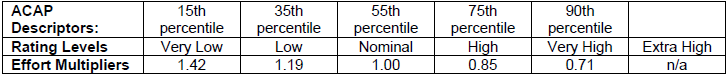
\includegraphics[width=\textwidth, height=0.4\textheight, keepaspectratio]{/home/francesco/git/Project_SE2_RTV/Project_Plan/PP_images/Acap.png}
\caption{ACAP}
\label{fig:ACAP}
\end{center}•
\end{figure}
\pagebreak
\item \underline{\textbf{Programmer Capability(PCAP)}}: The ability of our team is not only to be identified in the development from scratch but also in the use of APIs and services of third parties, which is why, despite the team's knowledge may not be high in any sphere, the high degree of dialogue and self-critical learning allow to better manage any eventuality. For this reason we define an \emph{HIGH} level.
\begin{figure}[h]
\begin{center}
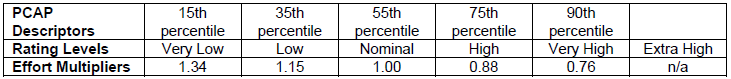
\includegraphics[width=\textwidth, height=0.4\textheight, keepaspectratio]{/home/francesco/git/Project_SE2_RTV/Project_Plan/PP_images/Pcap.png}
\caption{PCAP}
\label{fig:PCAP}
\end{center}•
\end{figure}
\linebreak
\item \underline{\textbf{Personnel Continuity (PCON)}}: This rating is in terms of the project’s annual personnel turnover. In particular, our team is composed by a limited number of people, and the possible turnover is very limited: so we assign a \emph{VERY HIGH} value.
\begin{figure}[h]
\begin{center}
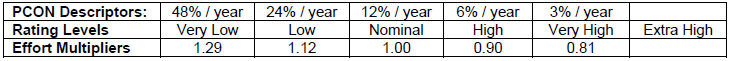
\includegraphics[width=\textwidth, height=0.4\textheight, keepaspectratio]{/home/francesco/git/Project_SE2_RTV/Project_Plan/PP_images/Pcon.png}
\caption{PCON}
\label{fig:PCON}
\end{center}•
\end{figure}
\linebreak
\item \underline{\textbf{Required Software Reliability (RELY)}}: This is the measure of the extent to which the software must perform its intended function over a period of time. With respect to the PowerEnjoy system, a software failure could block the functioning of the entire car sharing system, causing great losses in terms of money and image for the company. This driver cost is set to \emph{HIGH}.
\begin{figure}[h]
\begin{center}
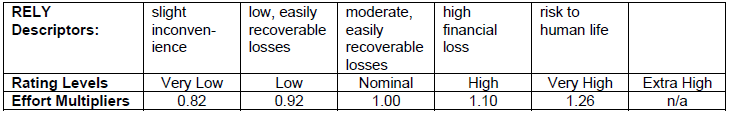
\includegraphics[width=\textwidth, height=0.4\textheight, keepaspectratio]{/home/francesco/git/Project_SE2_RTV/Project_Plan/PP_images/Rely.png}
\caption{RELY}
\label{fig:RELY}
\end{center}•
\end{figure}
\pagebreak
\item \underline{\textbf{Database Size (DATA)}}: This cost driver attempts to capture the effect large test data requirements have on product development. The rating is determined by calculating D/P, the ratio of bytes in the testing database to SLOC in the program. Since the car sharing service produces a high amount of information, divided between data relating to reservations, payments, users subscribed and other factors, given the amount of  SLOC computed before, we can assign the value \emph{VERY HIGH}.
\begin{figure}[h]
\begin{center}
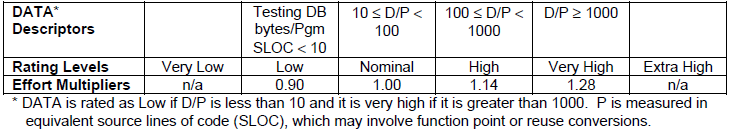
\includegraphics[width=\textwidth, height=0.4\textheight, keepaspectratio]{/home/francesco/git/Project_SE2_RTV/Project_Plan/PP_images/Data.png}
\caption{DATA}
\label{fig:DATA}
\end{center}•
\end{figure}
\pagebreak
\item \underline{\textbf{Product Complexity (CPLX)}}: With respect to the COCOMO II definition of this parameter, defined by the usage of the following tables, we assign the \emph{NOMINAL} level.
\begin{figure}[h]
\begin{center}
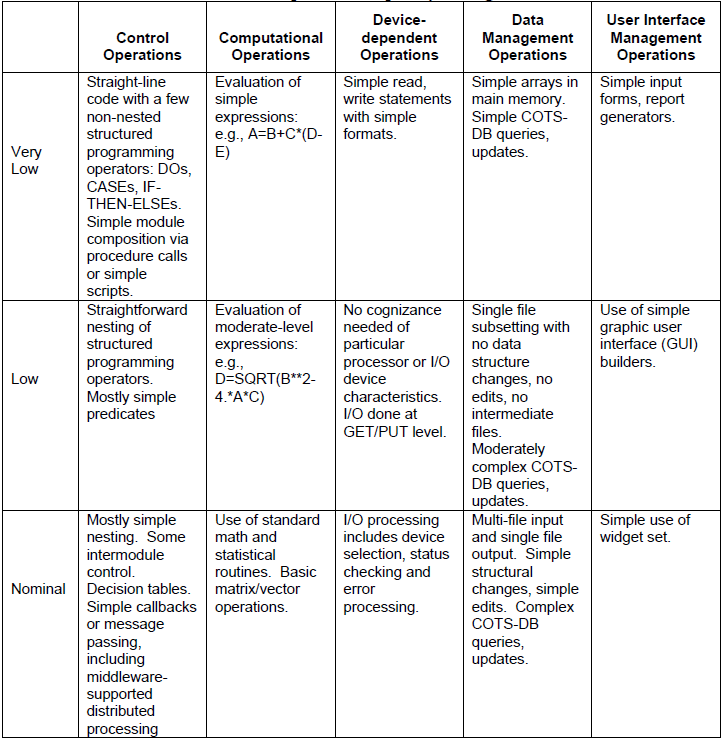
\includegraphics[width=\textwidth, height=0.8\textheight, keepaspectratio]{/home/francesco/git/Project_SE2_RTV/Project_Plan/PP_images/Cplx1.png}
\caption{CPLX1}
\label{fig:CPLX1}
\end{center}•
\end{figure}
\begin{figure}[h]
\begin{center}
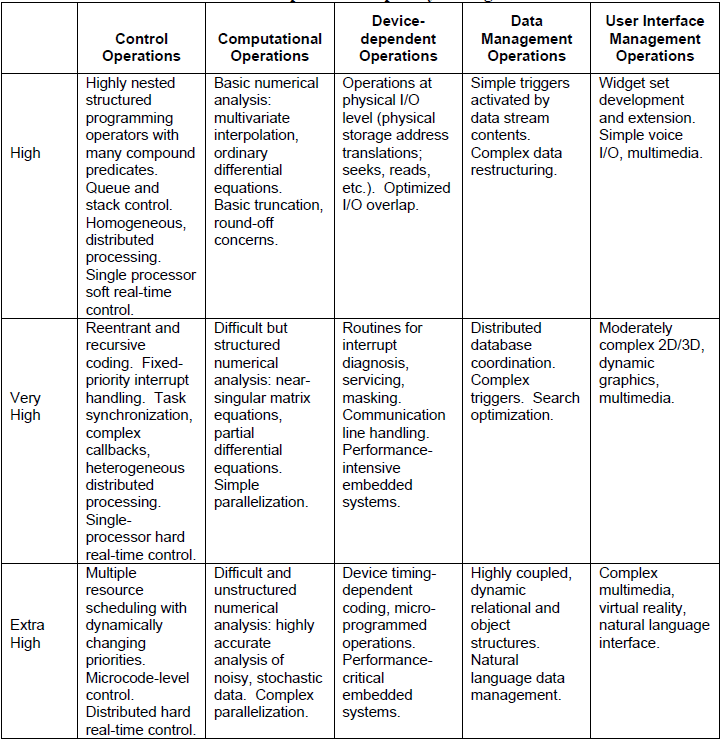
\includegraphics[width=\textwidth, height=0.8\textheight, keepaspectratio]{/home/francesco/git/Project_SE2_RTV/Project_Plan/PP_images/Cplx2.png}
\caption{CPLX2}
\label{fig:CPLX2}
\end{center}•
\end{figure}
\begin{figure}[h]
\begin{center}
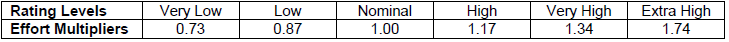
\includegraphics[width=\textwidth, height=0.4\textheight, keepaspectratio]{/home/francesco/git/Project_SE2_RTV/Project_Plan/PP_images/Cplx3.png}
\caption{CPLX3}
\label{fig:CPLX3}
\end{center}•
\end{figure}
\clearpage
\item \underline{\textbf{Documentation match to life-cycle needs (DOCU)}}: The rating scale for the DOCU cost driver is evaluated in terms of the suitability of the project’s documentation to its life-cycle needs; with respect to our system the documentation provided is complete and cover all the necessary elements of the life-cycle, from the requirements analysis to the integration testing. For this reason we assign a \emph{NOMINAL} level.
\begin{figure}[h]
\begin{center}
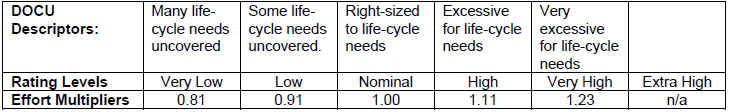
\includegraphics[width=\textwidth, height=0.4\textheight, keepaspectratio]{/home/francesco/git/Project_SE2_RTV/Project_Plan/PP_images/Docu.png}
\caption{DOCU}
\label{fig:DOCU}
\end{center}•
\end{figure}
\linebreak
\item \underline{\textbf{Developed for Reusability (RUSE)}}: This cost driver reflects the additional effort needed to construct components intended for reuse on current or future projects. In particular, our components are strictly linked with the project itself but are designed in order to be expandable for future evolution of the service. Despite those consideration, however, we have decided to invest some effort in order to detect functionalities which are evidently (and so easily) generalizable for using across programs. We assign a \emph{HIGH} value.
\begin{figure}[h]
\begin{center}
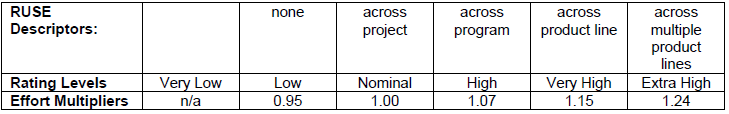
\includegraphics[width=\textwidth, height=0.4\textheight, keepaspectratio]{/home/francesco/git/Project_SE2_RTV/Project_Plan/PP_images/Ruse.png}
\caption{RUSE}
\label{fig:RUSE}
\end{center}•
\end{figure}
\pagebreak
\item \underline{\textbf{Execution Time Constraint (TIME)}}: This cost driver reflect the time constraint imposed upon the software system, in particular it express the percentage of available execution time expected to be used by the system. Since the car sharing is a 24h/7days service, we suppose to have an average level of usage (average in terms of different time of the day, for example) set to \emph{VERY HIGH}, since we expect to have a large number of users connected and using the system.
\begin{figure}[h]
\begin{center}
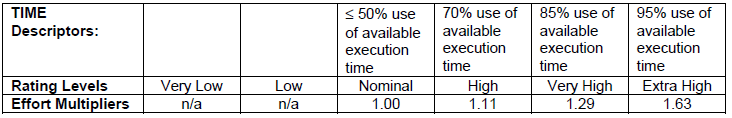
\includegraphics[width=\textwidth, height=0.4\textheight, keepaspectratio]{/home/francesco/git/Project_SE2_RTV/Project_Plan/PP_images/Time.png}
\caption{TIME}
\label{fig:TIME}
\end{center}•
\end{figure}
\linebreak
\item \underline{\textbf{Main storage constraint (STOR)}}: This parameter reflects the expected amount of storage usage with respect to the availability of the hardware. Our system produces a huge amount of data every day but since the increasing dimension of disk storage availability in these years, we set this value to \emph{NOMINAL}.
\begin{figure}[h]
\begin{center}
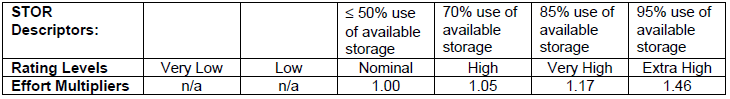
\includegraphics[width=\textwidth, height=0.4\textheight, keepaspectratio]{/home/francesco/git/Project_SE2_RTV/Project_Plan/PP_images/Stor.png}
\caption{STOR}
\label{fig:STOR}
\end{center}•
\end{figure}
\pagebreak
\item \underline{\textbf{Platform Volatility (PVOL)}}: This parameter points out the possible need to make updates to the system platforms, both hardware and software. In the short term there are no structural changes, however, you may need to update the user interface in case of the introduction of new features. We expect to implement new update on a \emph{HIGH} level.
\begin{figure}[h]
\begin{center}
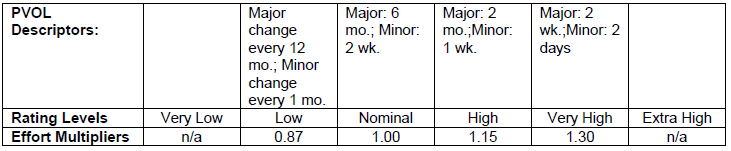
\includegraphics[width=\textwidth, height=0.4\textheight, keepaspectratio]{/home/francesco/git/Project_SE2_RTV/Project_Plan/PP_images/Pvol.png}
\caption{PVOL}
\label{fig:PVOL}
\end{center}•
\end{figure}
\linebreak
\item \underline{\textbf{Application Experience (APEX)}}: This driver is defined in terms of the project team level of experience with this type of application. Since is the first time, speaking for each member, to manage and develop an application with this dimension and amount of functionalities, the experience is limited to the 6 months of course lessons. We assign the \emph{LOW} value.
\begin{figure}[h]
\begin{center}
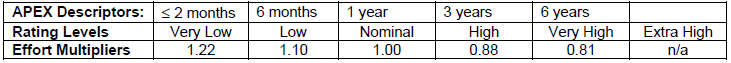
\includegraphics[width=\textwidth, height=0.4\textheight, keepaspectratio]{/home/francesco/git/Project_SE2_RTV/Project_Plan/PP_images/Apex.png}
\caption{APEX}
\label{fig:APEX}
\end{center}•
\end{figure}
\linebreak
\item \underline{\textbf{Platform Experience (PLEX)}}: The team has some previous experience in database management, user interfaces, client-server approach. The average knowledge about this kind of experience is comparable with a year so, with respect to the following table, we assign the value \emph{NOMINAL}.
\begin{figure}[h]
\begin{center}
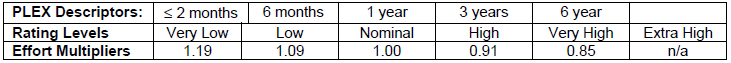
\includegraphics[width=\textwidth, height=0.4\textheight, keepaspectratio]{/home/francesco/git/Project_SE2_RTV/Project_Plan/PP_images/Plex.png}
\caption{PLEX}
\label{fig:PLEX}
\end{center}•
\end{figure}
\pagebreak
\item \underline{\textbf{Language and Tool experience (LTEX)}}: This parameter reflects the knowledge of the team about languages and tools that will be used in the system development. With respect to java language, J2EE, HTML and CSS the average knowledge of the team is a strong underground knowledge comparable with about 3 years. We set this value to \emph{HIGH}.
\begin{figure}[h]
\begin{center}
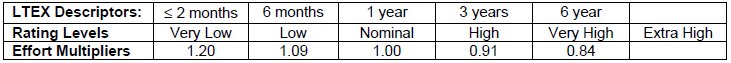
\includegraphics[width=\textwidth, height=0.4\textheight, keepaspectratio]{/home/francesco/git/Project_SE2_RTV/Project_Plan/PP_images/Ltex.png}
\caption{LTEX}
\label{fig:LTEX}
\end{center}•
\end{figure}
\linebreak
\item \underline{\textbf{Use of software tools (TOOL)}}: This parameter underlines the importance of the usage of tools well integrated in the environment in which the system is developed. Since our application make use of mature tools (as expressed in the architectural design in DD), we set this value to \emph{HIGH}.
\begin{figure}[h]
\begin{center}
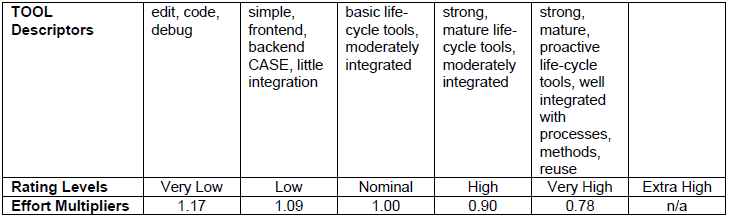
\includegraphics[width=\textwidth, height=0.4\textheight, keepaspectratio]{/home/francesco/git/Project_SE2_RTV/Project_Plan/PP_images/Tool.png}
\caption{TOOL}
\label{fig:TOOL}
\end{center}•
\end{figure}
\pagebreak
\item \underline{\textbf{Multisite development (SITE)}}: The development project has taken place mainly in remote, the team members has been kept informed each other regularly in case of autonomous work, however, the team has preferred to use conferencing tools to communicate and address the most important issues. For this reason we assign a \emph{VERY HIGH} value.
\begin{figure}[h]
\begin{center}
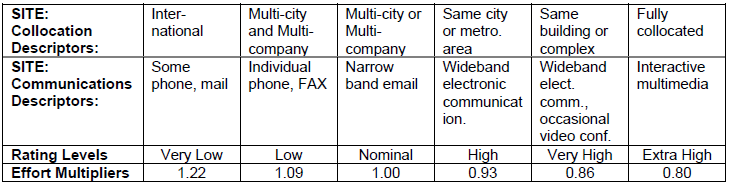
\includegraphics[width=\textwidth, height=0.4\textheight, keepaspectratio]{/home/francesco/git/Project_SE2_RTV/Project_Plan/PP_images/Site.png}
\caption{SITE}
\label{fig:SITE}
\end{center}•
\end{figure}
\linebreak
\item \underline{\textbf{Requirement development schedule (SCED)}}: This rating measures the schedule constraint imposed on the project team developing the software, in our particular case there were set strict deadline, so the schedule could not be relaxed, so we set the value to \emph{NOMINAL}.
\begin{figure}[h]
\begin{center}
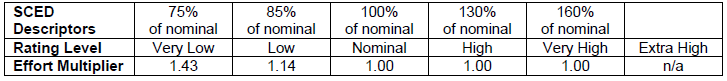
\includegraphics[width=\textwidth, height=0.4\textheight, keepaspectratio]{/home/francesco/git/Project_SE2_RTV/Project_Plan/PP_images/Sced.png}
\caption{SCED}
\label{fig:SCED}
\end{center}•
\end{figure}
\pagebreak
\end{itemize}
We now summarize all the selected cost drivers:
\begin{table}[h]
\caption{Cost drivers}
\begin{tabularx}{\textwidth}{|>{\hsize=.5\hsize}X|>{\hsize=.25\hsize}X|>{\hsize=.25\hsize}X|}
\hline
Cost driver & Factor & Value\\ 
\hline
Analyst Capability (ACAP) & High & 0.85\\
\hline
Programmer Capability(PCAP) & High & 0.88\\
\hline
Personnel Continuity (PCON) & Very High & 0.81\\
\hline
Required Software Reliability (RELY) & High & 1.10\\
\hline
Database size (DATA) & Very High & 1.28\\
\hline
Product Complexity (CPLX) & Nominal & 1.00\\
\hline
Documentation match to life-cycle needs (DOCU) & Nominal & 1.00\\
\hline
Developed for Reusability (RUSE) & High & 1.07\\
\hline
Execution Time Constraint (TIME) & Very High & 1.29\\
\hline
Main storage constraint (STOR) & Nominal & 1.00\\
\hline
Platform Volatility (PVOL) & High & 1.15\\
\hline
Application Experience (APEX) & Low & 1.10\\
\hline
Platform Experience (PLEX) & Nominal & 1.00\\
\hline
Language and Tool experience (LTEX) & High & 0.91\\
\hline
Use of software tools (TOOL) & High & 0.9\\
\hline
Multisite development (SITE) & High & 0.93\\
\hline
Requirement development schedule (SCED) & Nominal & 1.00\\
\hline
& Product & 1.135\\
\hline
\end{tabularx}
\end{table}
\pagebreak
\subsubsection{Effort equation}
We are now able to perform the effort equation expressed in paragraph 2.2 that we now rewrite with the computed coefficients:
\begin{center}
PM=A$\times$Size$^E\times\prod_{1<=i<=n}EM_i$
\end{center}
\begin{itemize}
\item A = 2.94
\item Average Size=9,614KSLOC;  Upperbound Size= 14,003KSLOC;
\item $\prod_{1<=i<=n}EM_i$ = 1.135
\item E = 1.0761
\end{itemize}
So:
\begin{itemize}
\item Average PM = 38.11 person-months
\item UpperBound PM = 57.12 person-months
\end{itemize}•
\subsubsection{Schedule estimation}
The duration of the project schedule is computed using the following equation:
\begin{center}
Duration=3.67$\times$PM$^{0.28+0.2\times(E-B)}$
\end{center}
Where:
B is equal to 0.91 for COCOMO II 
E is equal to 1.0761, computed as function of the scale factors, as above
PM is the effort computed with the effort equation at paragraph 2.2.3.
So we obtain:
\begin{itemize}
\item Average duration = 11.48 months $\simeq$ 12 months
\item Upperbound Duration= 13,03 months $\simeq$ 14 months
\end{itemize}•
\pagebreak
\section{Schedule}
In this chapter we’re going to define a high-level schedule for the project.
It’s important to underline that the result of this schedule should not be considered as defined and unchangeable, primarily because of the unforeseen that could occur (see chapter related to Risk Management) and may not ensure the timely achievement of milestones. Another reason is that it may also be necessary to return to work on previous task in case of possible adjustments.
\begin{enumerate}
\item We now define the main tasks to be scheduled:
\item Meetings with stakeholders: in order to give a first definition of requirements and features that the system-to-be must implement.
\item Requirement analysis and specification document (rasd): definition of a first document containing a detailed description of all requirements (functional and non-funcional) and goals related to the project.
\item Design Document (DD): definito of a first document describing the architectural design chosen for the development of the system.
\item Integration test plan document (ITPD): definition of a first document containing the sequence of integration and procedure necessary to cover the integration testing of the components of the system.
\item Project Plan Document (PPD): definition of a first document containing an analys of the possible dimension of the project, an estimation of the effort and cost, the schedule, the resource allocation and the risk management for the project.
\item Development: Development of the software system
\item Integration Test: Integration testing of the software system
\item Deployment: Deliver and deployment of the software to the customers.
\end{enumerate}
\textbf{NB}: The PP document is listed after the Design Document and not before because we are assuming that RASD and DD are already available and we could base this document also on what it’s written on them.
To compute the following schedule, we used all data retrieved from the analysis in this document and the duration of the drafting of the previous documents; in particular, we assumed that the team will work 8 hours per day (so the deadlines of the real project do not coincide with the one related to the course) excluding 2 days a week.
\pagebreak
\begin{figure}[h]
\begin{center}
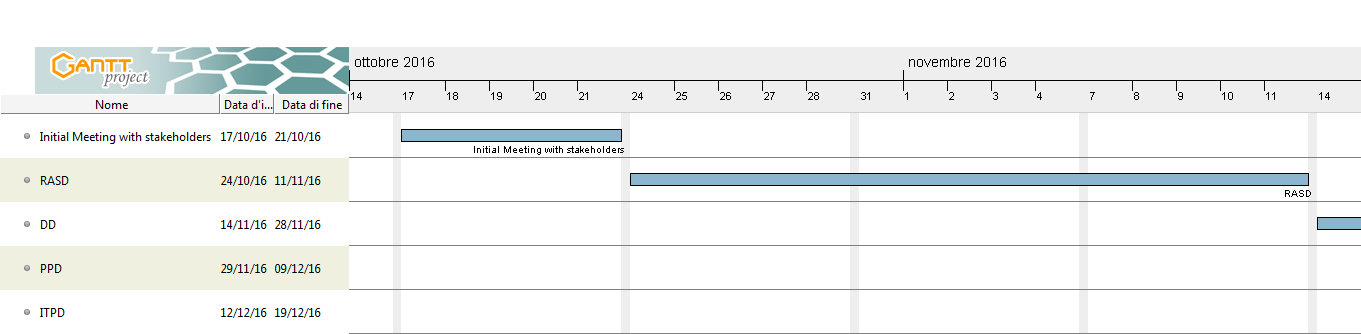
\includegraphics[width=\textwidth, height=0.8\textheight, keepaspectratio]{/home/francesco/git/Project_SE2_RTV/Project_Plan/PP_images/documentRA.png}
\label{fig:RASD}
\end{center}•
\end{figure}
\begin{figure}[h]
\begin{center}
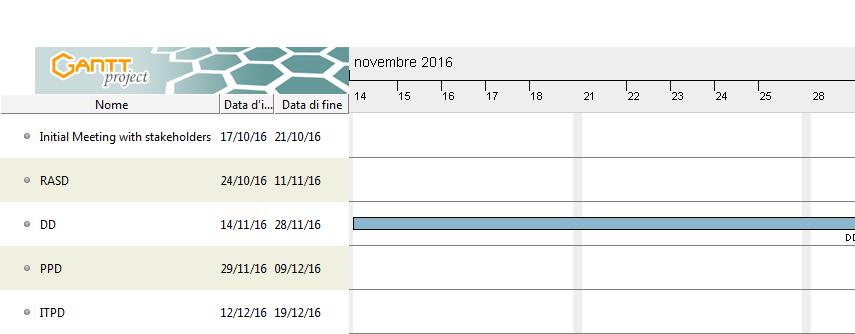
\includegraphics[width=\textwidth, height=0.8\textheight, keepaspectratio]{/home/francesco/git/Project_SE2_RTV/Project_Plan/PP_images/document.png}
\label{fig:DD}
\end{center}•
\end{figure}
\begin{figure}[h]
\begin{center}
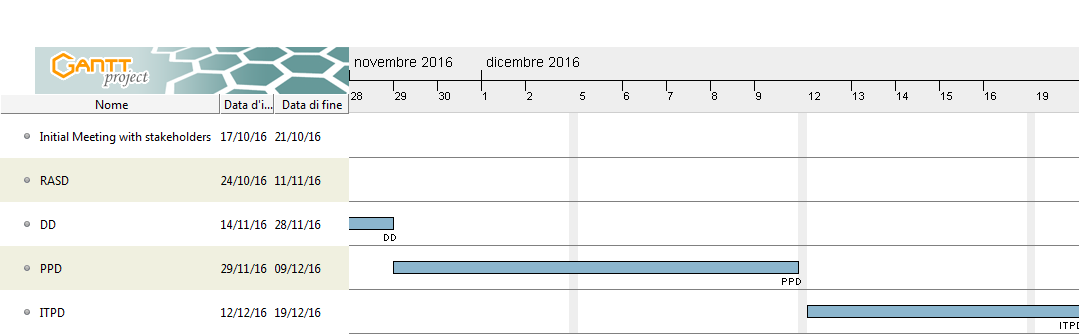
\includegraphics[width=\textwidth, height=0.8\textheight, keepaspectratio]{/home/francesco/git/Project_SE2_RTV/Project_Plan/PP_images/documentPPDITPD.png}
\label{fig:PPDITPD}
\end{center}•
\end{figure}
\begin{figure}[h]
\begin{center}
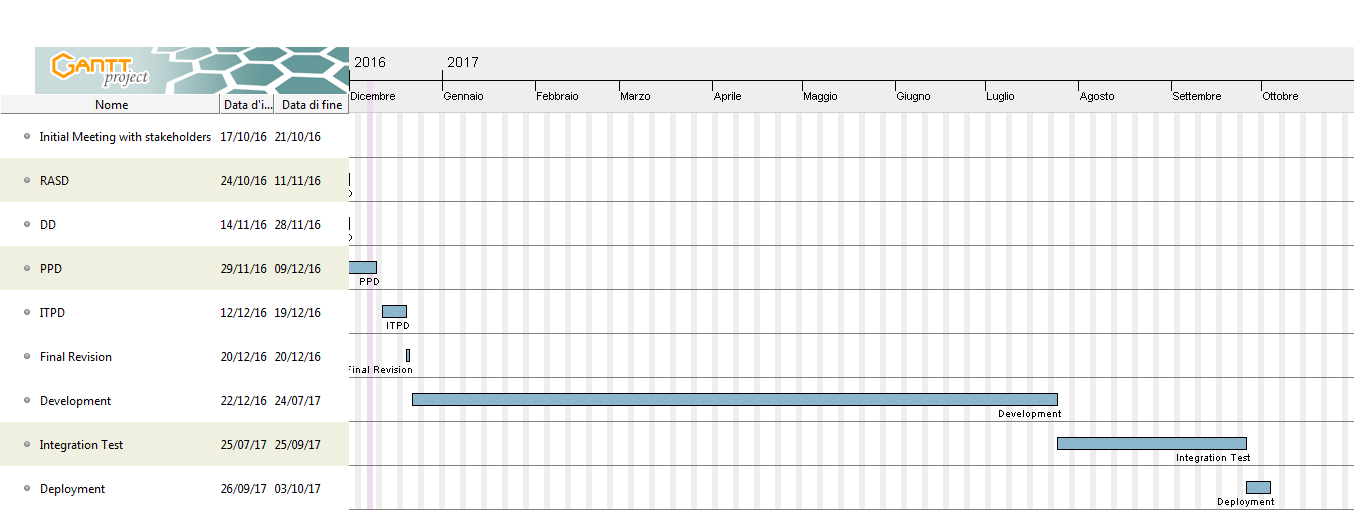
\includegraphics[width=\textwidth, height=0.8\textheight, keepaspectratio]{/home/francesco/git/Project_SE2_RTV/Project_Plan/PP_images/documentDevelopment.png}
\label{fig:DEV}
\end{center}•
\end{figure}
\clearpage
\section{Resource allocation}
In this paragraph we present the different steps that leads to the completion of all documents.
\begin{table}[h]
\caption{Resource allocation}
\begin{tabularx}{\textwidth}{|>{\hsize=.25\hsize}X|>{\hsize=.75\hsize}X|}
\hline
Document & Step\\
\hline
 & 1 - Meeting with stakeholders\\
\hline
RASD & 2 -Discussion defining requirements\\
\hline
 & 3 - Discussion defining Goals and Text assumptions\\
\hline
 & 4 - Constraints Definitions\\
\hline
 & 5 - Functional Requirements\\
\hline
 & 6 - Non Functional Requirements\\
\hline
 & 7 - Meetings with stakeholders in order to check the requirements\\
\hline
 & 8 - Scenarios\\
\hline
 & 9 - Brief revision to check what has been done\\
\hline
 & 10 - Use Case and Class Diagram\\
\hline
 & 11 - Sequence, Activity and State Diagram \\
\hline
 & 12 - Brief revision to check what has been done\\
\hline
 & 13 - Alloy Modeling\\
\hline
 & 14 - Copy Word File into a \LaTeX Document\\
\hline
 & 15 - Last revision on RASD\\
\hline
DD & 16 - Discussion defining Components and High-Level Components\\
\hline
& 17 - High-Level Components Diagram\\
\hline
& 18 - Component View Diagram\\
\hline
& 19 - Discussion defining Database entities and database components\\
\hline
& 20 - E-R Diagram\\
\hline
& 21 - Deployment View Diagram and Style Architecture Patterns\\
\hline
& 22 - Runtime Diagram\\
\hline
& 23 - Component Interfaces\\
\hline
& 24 - Brief revision to check what has been done\\
\hline
& 25 - Discussion concerning algorithm\\
\hline
& 26 - Algorithms Design\\
\hline
& 27 - Mockups \\
\hline
& 28 - Meetings with people in order to valuate the goodness of User Interface's Mockups\\
\hline
& 29 - UX Diagrams\\
\hline
& 30 - APIs and Requirements Traceability\\
\hline
& 31 - Copy Word File into a \LaTeX Document\\
\hline
& 32 - Last revision on DD\\
\hline
\end{tabularx}
\end{table}
\begin{table}[h]
\begin{tabularx}{\textwidth}{|>{\hsize=.25\hsize}X|>{\hsize=.75\hsize}X|}
\hline
ITPD & 33 - Discussion on what kind of integration strategy adopt\\
\hline
& 34 - Discussion on Identifying individual steps of component integration\\
\hline
& 35 - Integration Strategy\\
\hline
& 36 - Individual Steps and Test Description\\
\hline
& 37 - Brief revision to check what has been done\\
\hline
& 38 - Discussion on drivers\\
\hline
& 39 - Tools and Test Equipment\\
\hline
& 40 - Driver description\\
\hline
& 41 - Copy Word File into a \LaTeX Document\\
\hline
& 42 - Last revision on ITPD\\
\hline
PPD & 43 - Discussion on dispatching components into ILF, EIF, EI, EO, EQ\\
\hline
& 44 - ILF and EIF FPs evaluation and description \\
\hline
& 45 - EI, EO and EQ FPs evaluation and description\\
\hline
& 46 - Brief revision to check what has been done\\
\hline
& 47 - COCOMO II cost and effort estimation\\
\hline
& 48 - Brief revision to check what has been done\\
\hline
& 49 - Scheduling Plan\\
\hline
& 50 - Resource Plan\\
\hline
& 51 - Discussion on identifying what type of risks could affect the system\\
\hline
& 52 - Risk Management\\
\hline
& 53 - Copy Word File into a \LaTeX Document\\
\hline
& 54 - Last revision on PPD\\
\hline
\end{tabularx}
\end{table}
\begin{figure}[h]
\begin{center}
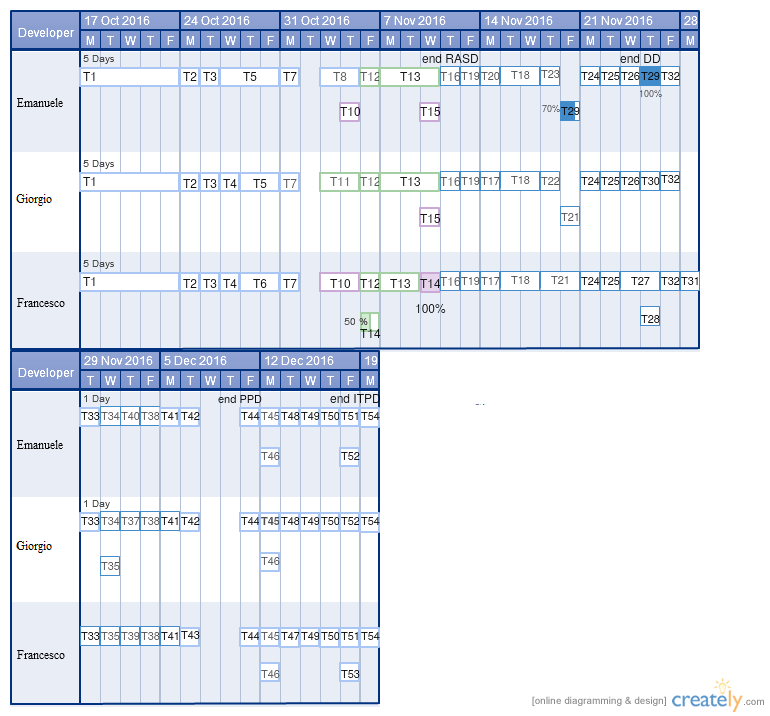
\includegraphics[width=\textwidth, height=0.7\textheight, keepaspectratio]{/home/francesco/git/Project_SE2_RTV/Project_Plan/PP_images/staff_powerenjoy.png}
\label{fig:RES}
\end{center}•
\end{figure}
\clearpage
\section{Risk management}
This chapter will face the risk management related to the development of the PowerEnJoy system, in particular, we will try to identify the main risks that the development could come up against and, for each of them, we’ll define some behaviours to apply before, to prevent the concrete risk, or after the actual hit to face it the best way.
The first possible risk in which development might bump, is constituted by a change of the requirements and features to be implemented in the system, in progress of development. The first solution to solve this possibility is given by the construction of an architecture elastic, able to grant a large margin of changes and improvement (also in view of future updates); However, this should not be seen as the only solution to be taken as a continuous or sudden change in requirements can lead to problems of misunderstanding between teams and stakeholders, as well as within the team itself.
For this reason, it is very important to prevent these possibilities maintaining a constant dialogue with stakeholders. Allowing them to verify the state of development of each functionality, thus also providing practical examples of immediate understanding in order to obtain the maximum possible agreement, in the event that changes were required, these may be implemented in the course of work.
Another aspect related to the concept of collaboration and dialogue between stakeholders and team leads us to consider the problem of the response to the final user.
In particular, we must take into account that nowadays the car sharing services are widespread, and that users prefer a service rather than another both for economic reasons and for simplicity in using the service’s user interface. In our case, this results in the development of a user friendly interface for the application, in order to make the best choices and user preferable, it is therefore advisable to carry out meetings with future users, randomly selected, and carefully study their feedback, focusing these meetings especially just before the release, with briefings or small interview asking what kind of environment the user is looking for.
Earlier we mentioned the team and how certain factors can influence the development negatively.
One of the problems that may be encountered is the lack of understanding. This may be due to multiple reasons, primarily due to the lack, or rare, presence of internal meetings: these in fact not only guarantee to maintain an updated flow of informations about the state of development through the developing teams, but also to promote constant motivation and teamwork.
The misunderstanding may result from other factors, such as incohesive team, where the communication among its members is not proper, so a situation in which each member doesn’t know how is the working progress, is very common.
The choice of subdividing the work load through multiple teams (task subdivision) could be seen as a remedy in case of absence (illness or other reasons) of one of the members, so as not to slow down too much the development because they work on different tasks.
Continuing on the team's considerations, we can say that the development environment consists on mature programs, which therefore should not show any problems or obstacles to development. Same thing can be done with regard to google APIs used, which at most may go and introduce / remove the feature; for this reason you need to stay informed about updates and then be able to implement them as soon as possible, both during and after the development.
Although our team is equipped with the necessary knowledge for the development of this type of system, in order to avoid possible stalls or delays in the development of the more complex features of the system, it has been carried out a careful analysis at the beginning of the process, so as to ensure the recruitment of specialized staff (for limited periods) to remedy at these eventualities.
With regard to the maintenance company and the payment system, that are the outside companies with which we have made contracts for the management of particular fields, we must assume that these contracts may expire, and then the external companies may change. It is therefore necessary that our system is able to quickly interface with the new services, in order to minimize possible disruption of service: for this reason it is necessary to focus on the development of components as flexible as possible.
Another risk in which the development and especially the release system may encounter is constituted by the hardware, that is necessary for our system. 
In order to avoid reliability problems (due to the nature of the service) and also the increasing cost due to the wrong choice of maintaining the system by our own (more expensive), we have decided to move the system onto a cloud architecture, that maintains lower costs and ensures a constant and efficient service.
All these risks could slow down the achievement of one or more deadlines in the schedule, for this reason it is necessary to carry out an analysis of the same schedule in relation to risk management, so as to ensure safety margins. About this, we have counted few more hours in the Resource Planning to avoid that the slowing down of our work forces us to break the deadlines. We know that more working hours correspond to a more costly system for the customer, and taking care of that, the amount of surplus hours is the minimum necessary to allow the schedule to be more relaxed but however it does not too much burden the system cost. In that unlikely situation, we will release before the most important functionalities of our system and then we’ll progressively release the remaining part with upgrades.
\addcontentsline{toc}{section}{Used tools}
\section*{Used tools}
\begin{itemize}
\item Github: for version control
\item GoogleDoc: to write the document
\item Draw.io: to create the diagrams
\item \LaTeX: to create the pdf
\item Creately: for Resource Allocation diagram
\item Gantt Project: to create Gantt Diagrams
\end{itemize}
\addcontentsline{toc}{section}{Work hours}
\section*{Work hours} 
\begin{itemize}
\item Emanuele Ricciardelli: $\sim$ 30 hrs.
\item Giorgio Tavecchia: $\sim$ 30 hrs.
\item Francesco Vetr\'o: $\sim$ 30 hrs.
\end{itemize}
\end{document}


